\problemname{Astronom}
\illustration{.3}{img/TychoBrahe.JPG}{}

\noindent
% The astronomer has a passion for stargazing.
Pasją pewnego astronoma jest obserwacja gwiazd.
% In particular, he gets immense pleasure out of gazing at $k$~stars simultaneously through his telescope.   
W szczególności czerpie on ogromną przyjemność z wpatrywania się w $k$~gwiazd jednocześnie przez swój teleskop.   
% Building a telescope with radius~$r$ costs $t\cdot r$~kroner.
Budowa teleskopu o promieniu~$r$ kosztuje $t\cdot r$~koron.
% A newly built telescope will point exactly at the origin $(0,0)$.
Nowo zbudowany teleskop będzie wskazywał dokładnie na początek $(0,0)$.
% Moving it to point somewhere else also takes effort; 
Przesuwanie go tak, by wskazywał gdzie indziej, również wymaga wysiłku; 
% shifting the telescope a distance of $d$~units incurs a cost of $s\cdot d$~kroner.
przesunięcie teleskopu o odległość $d$~jednostek kosztuje $s\cdot d$~koron.
% The astronomer can observe all stars at distance at most $r$ from where the telescope points.
Astronom może obserwować wszystkie gwiazdy w odległości co najwyżej $r$ od miejsca, na które wskazuje teleskop.

% How much does it cost to build and move a telescope that allows $k$~stars to be observed at once?
Ile kosztuje zbudowanie i przesunięcie teleskopu, który umożliwia jednoczesną obserwację $k$~gwiazd?

\medskip

% All coordinates and distances are given in the Euclidean plane.
Wszystkie współrzędne i odległości podane są w płaszczyźnie euklidesowej.


\section*{Przykład}

% Here is an example with $n=3$ stars at positions $(0,0)$, $(2,0)$, and $(3,1)$.
Oto przykład z $n=3$ gwiazdami na pozycjach $(0,0)$, $(2,0)$ oraz $(3,1)$.
% The shaded area shows a telescope of radius~$1$ pointing at $(1,0)$ covering two stars; this costs $s + t$~kroner and is an optimal solution to sample input~$3$.
Zacieniowany obszar pokazuje teleskop o promieniu~$1$ skierowany na $(1,0)$ obejmujący dwie gwiazdy; kosztuje to $s + t$~koron i jest optymalnym rozwiązaniem dla przykładowego wejścia~$3$.
% The image also shows optimal solutions to sample inputs~$1$, $2$, and $4$.
Obraz pokazuje również optymalne rozwiązania dla przykładowych wejść~$1$, $2$ oraz $4$.

\medskip
\noindent
% \includegraphics\[width=.3\textwidth\]{img/samples.pdf}
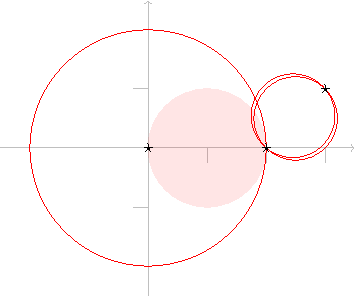
\includegraphics[width=.3\textwidth]{img/samples.pdf}


\section*{Wejście}

% The first line consists of four integers:
Pierwszy wiersz składa się z czterech liczb całkowitych:
% the number~$k$ of stars the astronomer wants to observe,
liczba~$k$ gwiazd, które astronom chce obserwować,
% the number~$n$ of stars in tonight's sky,
liczba~$n$ gwiazd na dzisiejszym niebie,
% the shifting cost~$s$, and
koszt przesunięcia~$s$, oraz
% the telescope building cost~$t$.
koszt budowy teleskopu~$t$.
% Then follow $n$ lines, where the $i$th line contains the integer coordinates $x_i$ and $y_i$ of the $i$th star.
Następnie znajduje się $n$ wierszy, gdzie $i$-ty wiersz zawiera współrzędne całkowite $x_i$ oraz $y_i$ gwiazdy o numerze $i$.

\section*{Wyjście}

% A single real number: the minimum number of kroner that the astronomer needs to spend.
Pojedyncza liczba rzeczywista: minimalna liczba koron, którą astronom musi wydać.

\section*{Ograniczenia i punktacja}

% You can assume 
Możesz założyć 
\begin{enumerate}
\item $1\leq k\leq n\leq 700$. % constraint:kn
\item $x_i, y_i\in \{-10^9,\ldots, 10^9\}$ dla każdego $i\in\{1,\ldots,n\}$. % constraint:xy
\item $s,t\in \{0,\ldots, 10^9\}$. % constraint:st
% \item Your output is accepted if it is within a relative or absolute tolerance of $\epsilon = 10^{-6}$ of the correct answer.
\item Twoja odpowiedź będzie zaakceptowana, jeśli mieści się w względnej lub bezwzględnej tolerancji $\epsilon = 10^{-6}$ od prawidłowej odpowiedzi.
\end{enumerate}


% Your solution will be tested on a set of test groups, each worth a number of points.
Twoje rozwiązanie zostanie przetestowane na zestawie grup testowych, z których każda jest warta pewną liczbę punktów.
% Each test group contains a set of test cases.
Każda grupa testowa zawiera zestaw przypadków testowych.
% To get the points for a test group you need to solve all test cases in the test group.
Aby uzyskać punkty za grupę testową musisz rozwiązać wszystkie przypadki testowe w tej grupie.
% Your final score will be the maximum score of a single submission.
Twój ostateczny wynik będzie maksymalnym wynikiem pojedynczego zgłoszenia.

\medskip
\noindent
\begin{tabular}{lll}
%   Group & Points & Constraints\\\hline
 Grupa & Punkty & Ograniczenia\\\hline
  $1$ & $8$ &  $t\leq s$\\
  $2$ & $9$ & $n\le 50$ oraz $s=0$\\
  $3$ & $18$ & $s=0$\\
  $4$ & $13$ & $n\leq 50$\\
  $5$ & $14$ & $n\leq 350$\\
  $6$ & $15$ & $\epsilon = 1/10$\\
%   $7$ & $23$ & \emph{No further constraints}\\
  $7$ & $23$ & \emph{Brak dodatkowych ograniczeń}\\
\end{tabular}
